\section*{Three exact finite models}\addcontentsline{toc}{section}{Three exact finite models}
\subsection*{A seed remembers multiplicity support}
For $M_2(\mathbb C)\otimes I_3$, a coefficient matrix with rank one generates a two-dimensional orbit. A rank-two matrix generates a four-dimensional orbit. Neither single seed spans the six-dimensional space, because a $2\times3$ matrix cannot have rank three. Two seeds can cover the three multiplicity coordinates together. This is the finite seed-rank formula with $d=2$ and $m=3$.
\begin{figure}[H]\centering
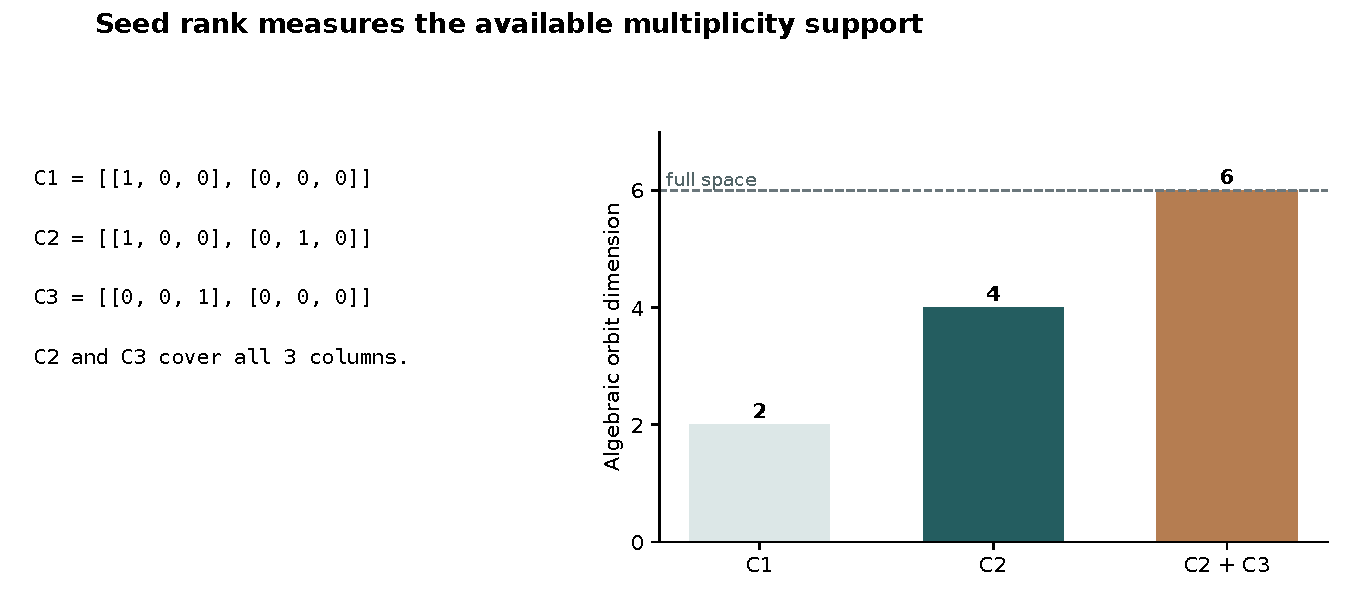
\includegraphics[width=.94\textwidth]{monograph_figures/exact_seed_support.pdf}
\caption{Exact coefficient matrices for $d=2$, $m=3$. The combined row support of two seeds has rank three. The bar heights are algebraic orbit dimensions, not unitary preparation probabilities.}\label{monograph:fig:seed_support}
\end{figure}
\clearpage
\subsection*{An eliminated coordinate still contributes}
Take $H=\left(\begin{smallmatrix}2&1\\1&3\end{smallmatrix}\right)$ and retain its first coordinate. The eliminated block is invertible and the Schur complement of $H$ is $2-1/3=5/3$. Its inverse is $3/5$, exactly the retained entry of $H^{-1}$. Inverting the compressed entry alone gives $1/2$. The difference comes from a path through the discarded coordinate.
\begin{figure}[H]\centering
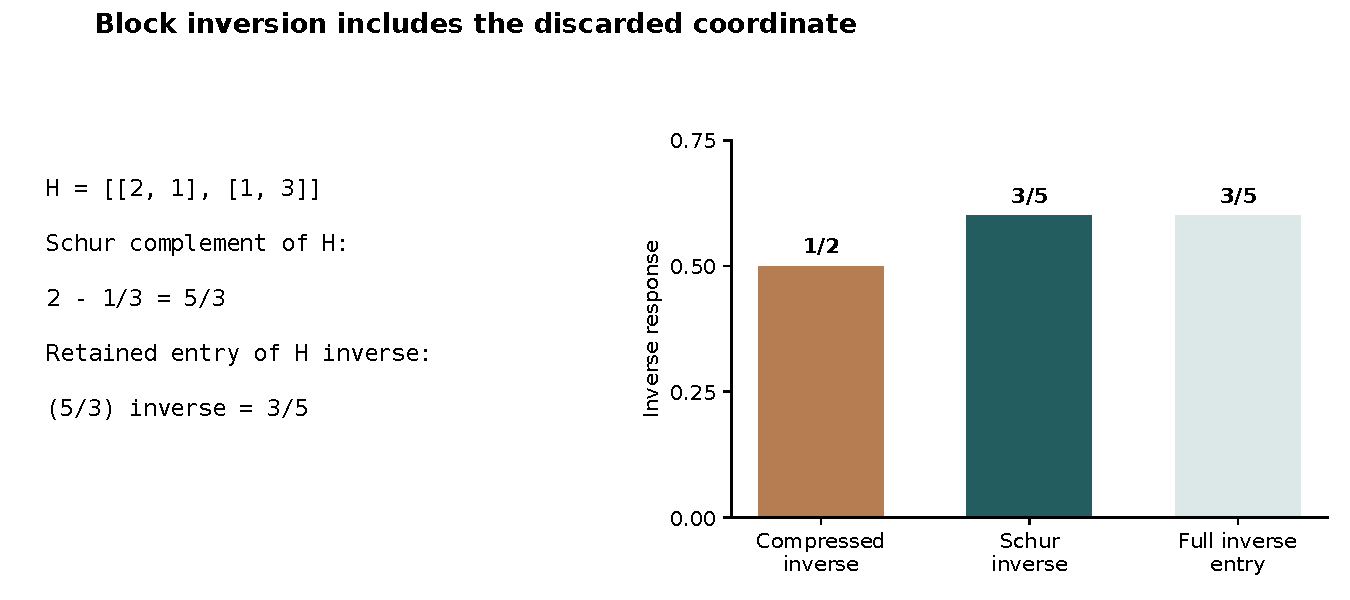
\includegraphics[width=.94\textwidth]{monograph_figures/exact_feshbach_compression.pdf}
\caption{A rational two-coordinate block-inverse model. Both the eliminated block and full operator are invertible. The plotted values are exact fractions. This example distinguishes direct compression from resolvent elimination.}\label{monograph:fig:feshbach_compression}
\end{figure}
\clearpage
\subsection*{Normalization changes the map}
Let $P=|0\rangle\langle0|$ on $\mathbb C^2$ and $Z=\operatorname{diag}(1,-1)$. The normalized Kraus family $\sqrt{3/4}\,I$, $\sqrt{1/4}\,Z$ satisfies $\sum_j K_j^*K_j=I$ and maps $P$ to $P$. The unnormalized family $\sqrt3\,I$, $Z$ satisfies $\sum_j E_j^*E_j=4I$ and maps $P$ to $4P$. The same relative weights produce different output traces.
\begin{figure}[H]\centering
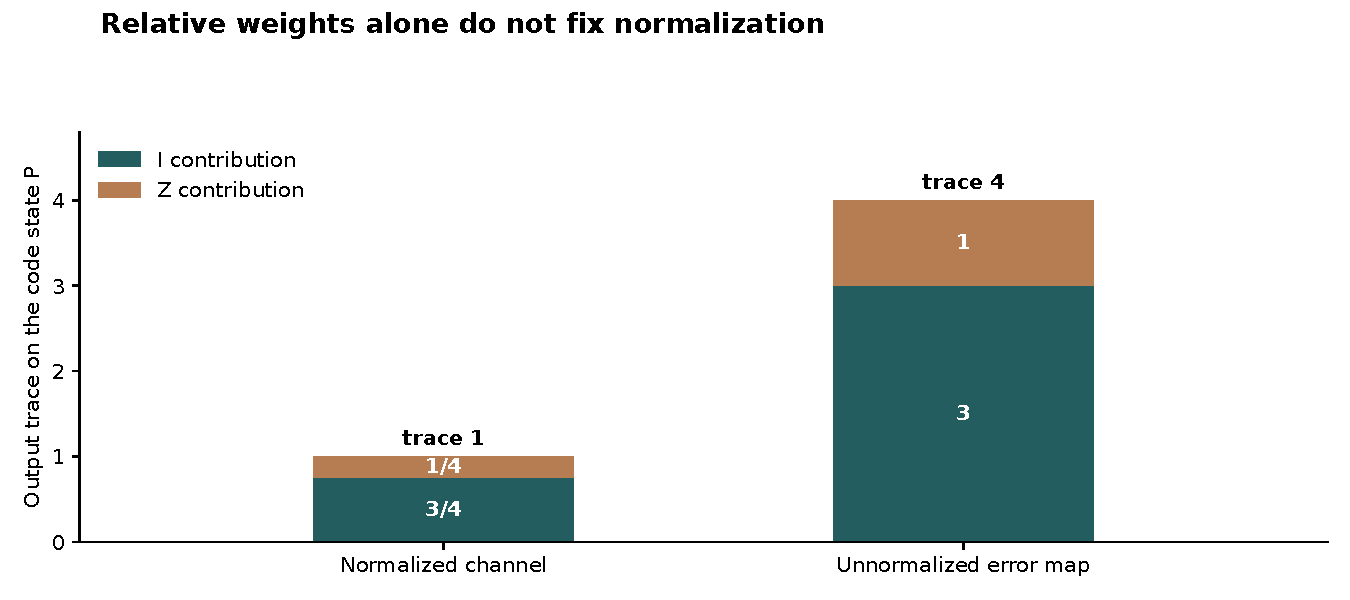
\includegraphics[width=.94\textwidth]{monograph_figures/exact_channel_scale.pdf}
\caption{Exact weights for one supported code state. The normalized map preserves trace one. The unnormalized positive map has output trace four. The illustration records this finite scaling distinction and does not assert a general recovery construction.}\label{monograph:fig:channel_scale}
\end{figure}
\clearpage
